На рисунке изображена упрощенная концептуальная модель того как распределяется наше виртуальное адресное пространство между тем что будет в этом адресном пространстве существовать.

\begin{figure}[htbp]
  \centering
  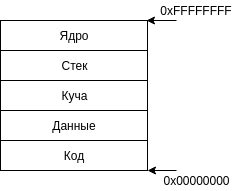
\includegraphics[width=0.3\textwidth]{./memory/memory-model/memory-model.png}
\end{figure}

По младшим адресам оперативной памяти, как мы уже говорили, располагается код ядра, за ним следует стек. Стек растет к младшим адресам. Положить данные на вершину стека можно с помощью операции push и забрать с вершины с помощью операции pop.

Дальше идет неиспользованное, свободное по умолчанию пространство, называемое кучей. Куча --- пространство между стеком и данными.

Коду приложения отводятся самые старшие адреса. Это пространство нужно для того, чтобы мы не могли случайно или специально поменять наш код и заставить это приложение работать по-другому.